\chapter{Evaluation}

\todo{Allgemeine Anmerkung: Ich finde es persoenlich bei diesen
Kapiteleinleitungen schoener, wenn die "section" immer am Anfang des satzes steht
damit man nicht vor und zurück springt. Aber das ist geschmackssache.}

In this chapter, experimental results are presented while setting
focus on different aspects.
Before evaluating the performance of the final localization algorithm the
\ac{WSDE} on single robots is examined by first taking a closer look
at a representative example in \cref{sec:04_tdoaSingle}.
There, the focus is set on the \ac{TDOA} methods itself for each channel pair
before combining them to a robot direction result.
\Cref{subsec:04_singleRobotAngleError} presents the validity of the methods with
regard to a whole set of data.

% Additional Info
In \cref{chap:03_implementation}, the presence of additional
information next to the estimated \ac{WSDE} on individual robots
is discussed.
This includes knowledge about \acp{SNR} of the channel signals, the \ac{PSNR}
of the \ac{GCC} functions and a distance approximation if the signal source
is detected straight in front or from behind.
\Cref{sec:04_additionalInformation} analyses if and to
what extent these factors are useful for the \ac{WSDE} or \ac{WSL}.

% Team filter
To examine the whistle sound source localization of the robots as team,
measurements were taken with five Naos on the field of the HULKs' laboratory
as specified in \cref{subsec:04_labMeasurements}.
In \cref{sec:04_teamEvaluation} the performance of the \ac{TDOA} methods are presented
and compared for all measurements.
Depending on the accuracy of the individual direction results, the quality
of the team filter is limited.
% Therefore, the angular error of the single robots is demonstrated for each
% measurement and method.

All measurements presented in this chapter were recorded in the
laboratory of the HULKs and are taken from a sound source at a height of
\SI{1.5}{\meter} above ground.
The size of the field used in this work is smaller than the regular \ac{SPL}
field with 7.5\si{m} length and 5\si{m} width instead of 9\si{\meter} and 6\si{\meter}.
This circumstances occur due to lack of space and limited size of the
field room in the laboratory.
Another deviation to competition conditions arise due to walls being next to field borders.
In \cref{subsec:04_labMeasurements} further information about the measurement setup
is introduced.

\subsection{Measurement Setup}
\label{subsec:04_labMeasurements}

Eleven measurement were taken with five robots on the small-sized \ac{SPL} field
of the HULKs laboratory.
\Cref{fig:04_setup} illustrates the positions of the NAO robots
and the positions of the whistle-sound sources.
% -------------------------------------------------------------
\begin{figure}[ht]
	\centering
		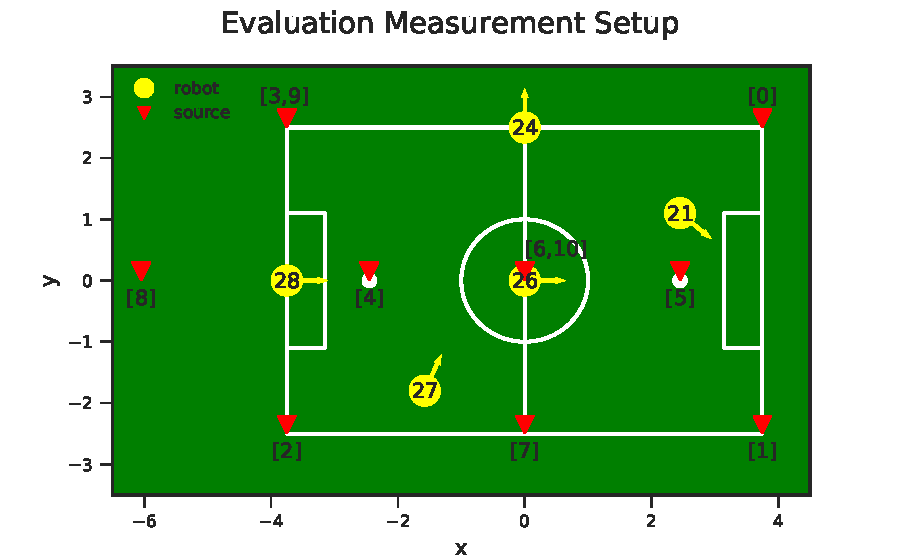
\includegraphics[]{figures/evaluation/setup}
	\caption{Setup of robots and sound source positions for the evaluation measurement.}
    \label{fig:04_setup}
\end{figure}
% -------------------------------------------------------------

According to these, the x- and y-coordinates of the sound source positions and
robots are listed in \cref{tab:04_robots} and \cref{tab:04_sources}, respectively.
Additionally, the positions are named for easier memorability.
The orientation $\theta$ of the robots are defined relatively to the global
x-axis as defined in \cref{subsec:03_coordinates}.
In the following, the measurements introduced in this section are
referred to as \textit{laboratory-dataset}.
% -------------------------------------------------------------
\btline{ht}{1.2}
\btab{|c|c|c|c|}
\hline
NAO & x [\si{m}] & y [\si{m}] & $\theta$ [\si{deg}]\\
\hline
21 & 3.75 & 2.5 & -40.2\\
\hline
24 & 3.75 & -2.5 & 90\\
\hline
26 & 0 & 0 & 0\\
\hline
27 & -3.75 & -2.5 & 66.06\\
\hline
28 & -2.45 & 0 & 0\\
\hline
\etab
\et{Robot positions of the laboratory-dataset}{04_robots}
% -------------------------------------------------------------
\btline{ht}{1.2}
\btab{|c|c|c|c|}
\hline
Measurement & Position Name & x [\si{m}] & y [\si{m}]\\
\hline
0 & front left & 3.75 & 2.5\\
\hline
1 & front right & 3.75 & -2.5\\
\hline
2 & rear right & -3.75 & -2.5\\
\hline
3.9 & rear left & -3.75 & 2.5\\
\hline
4 & own penalty spot & -2.45 & 0\\
\hline
5 & opponent penalty spot & 2.45 & 0\\
\hline
6.10 & center & 0 & 0\\
\hline
7 & center right & 0 & -2.5\\
\hline
8 & behind own goal & -6.05 & 0\\
\hline
\etab
\et{Positions of the whistle sources in the laboratory-dataset}{04_sources}
% -------------------------------------------------------------

\section{\acl{WSDE}}
\label{sec:04_tdoaSingle}

Before evaluating the performance of the different methods as a whole,
% For comparability of the results,
one exemplary measurement is utilized
to present and analyse the \ac{TDOA} methods in detail first.
In this recording, the sound source is placed at the right front
of the robot with 4.5\si{m} distance.
Hereinafter, this measurement will be referenced to as \textit{demonstration-dataset}.
This corresponds to an an angle of -33.7\si{\degree} in robot coordinates.
To get an idea about the examined data, according whistle signal samples around the
start are plotted in \cref{fig:04_tdoaSignal} for all channels.
% -------------------------------------------------------------
\begin{figure}[ht]
	\centering
		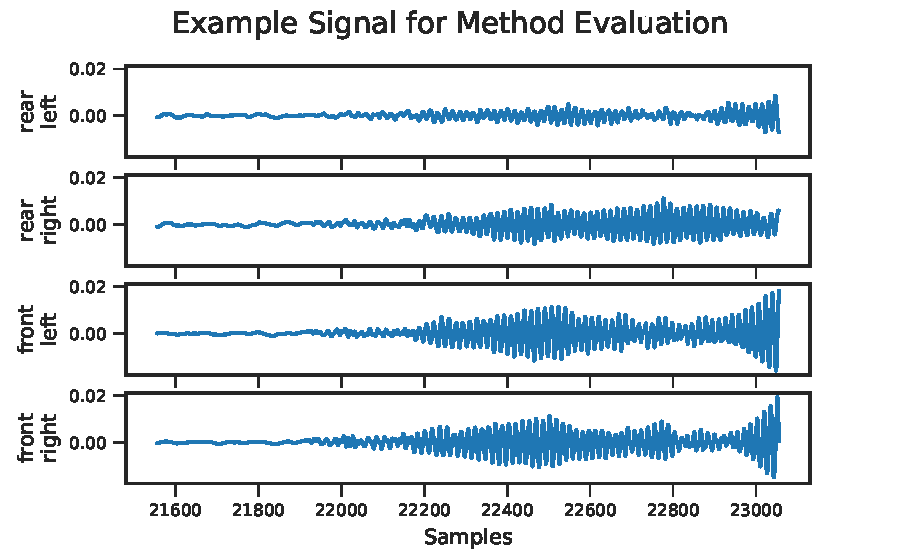
\includegraphics[]{figures/evaluation/cc_frontRight_1_signal}
	\caption{Signal start section of a whistle sound recorded from front right.}
	\label{fig:04_tdoaSignal}
\end{figure}
% -------------------------------------------------------------

As the next sections focus on the performance of the \ac{TDOA} methods,
the start index is set manually.

For the sake of conciseness, throughout the following sections the correlation
function $R_{x_ax_b}$ of two signals $x_a$ and $x_b$  (\cf
\cref{chap:02_prerequisites}) is denoted as $R_{ab}$.


\subsection{Cross Correlation}
\label{subsec:04_ccSingle}
% -------------------------------------------------------------

The \ac{CC} is a widespread technique to obtain the time delay
between two series of samples.
To discuss the result of the \ac{CC}, the belonging correlation functions
of the demonstration-dataset are plotted in \cref{fig:04_cc}.
The selection process and implementation correspond to the explanations
in \cref{subsubsec:03_cc}.
For $R_{32}$ and $R_{13}$ a peak is clearly visible.
However, for the other \ac{CC} the problem of a weak peak
arises what was mentioned as downside of the \ac{CC} in \cref{sec:02_cc}.
% -------------------------------------------------------------
\begin{figure}[ht]
	\centering
		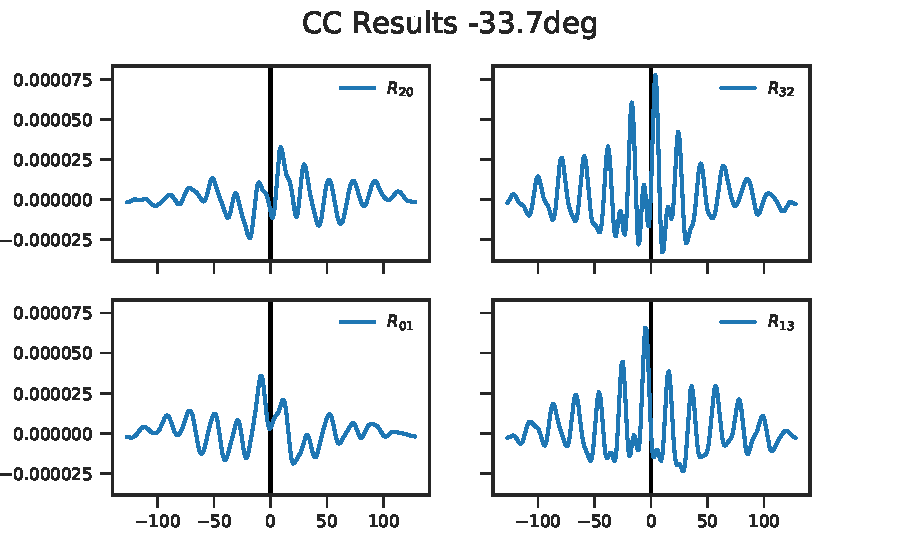
\includegraphics[]{figures/evaluation/cc_frontRight_1}
	\caption{Cross correlation results of signal from front right (-33.7\si{\degree}).}
	\label{fig:04_cc}
\end{figure}
% -------------------------------------------------------------
\btline{ht}{1.2}
\btab{|c|c|c|c|c|}
\hline
Base Channel & Next Channel & Delay & Candidate (-) & Candidate (+)\\
\hline
0 & 1 & -8.25 & -144.9 & -35.1\\
\hline
1 & 3 & -4.59 & -17.4 & 78.6\\
\hline
2 & 0 & 9.16 & -30.6 & -30.6\\
\hline
3 & 2 & 3.94 & -150.2 & -29.8\\
\hline
\etab
\et{Cross correlation delay results of signal from front right}{04_cc}
% -------------------------------------------------------------

According to the delays in \cref{tab:04_cc}, two source direction candidates arise
for each channel pair.
By the implementation in \cref{subsec:03_directionCandidates}, the combination of
all options with the smallest error is selected as \ac{WSDE}.
Hence, the algorithm outputs -26.9\si{\degree} what produces an error of 6.8\si{\degree}.
The delay between channel 2 and 0 is larger than the maximum delay of 6.85 samples
and therefore cut to the maximum sample delay.
Besides these, the \ac{TDOA} between the channel pairs produce one appropriate
direction candidate which correctly points to the sound source.
% -------------------------------------------------------------

\subsection{Generalized Cross Correlation}
\label{subsec:04_gccSingle}
% -------------------------------------------------------------
\Cref{fig:04_gcc} presents the \ac{GCC} result by the \ac{GCC-PHAT} method of
the demonstration-dataset equal to \cref{subsec:04_ccSingle}.
The subsample delays for each channel pair and their resulting direction candidates
are listed in \cref{tab:04_gcc}.
From this, a final direction of -30.0\si{\degree} is determined
resulting in an error of 3.69\si{\degree}.
It is apparent that the peaks of the \ac{GCC} are better to detect than the peaks of the
\ac{CC}.
% -------------------------------------------------------------
\begin{figure}[ht]
	\centering
		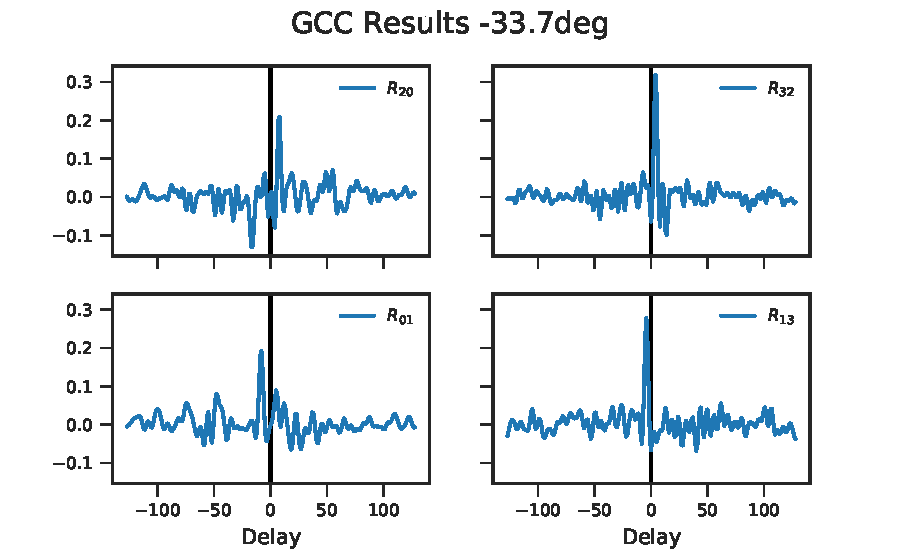
\includegraphics[]{figures/evaluation/gcc_frontRight}
	\caption{Generalized cross correlation results of signal from front right.}
	\label{fig:04_gcc}
\end{figure}
% -------------------------------------------------------------
\btline{ht}{1.2}
\btab{|c|c|c|c|c|}
\hline
Base Channel & Next Channel & Delay & Candidate (-) & Candidate (+)\\
\hline
0 & 1 & -8.28 & -144.7 & -35.3\\
\hline
1 & 3 & -4.09 & -22.8 & 84.0\\
\hline
2 & 0 & 7.60 & -30.6 & -30.6\\
\hline
3 & 2 & 4.13 & -148.7 & -31.3\\
\hline
\etab
\et{Generalized cross correlation delay results of signal from front right}{04_gcc}
% -------------------------------------------------------------
\subsection{Phase Difference}
\label{subsec:04_phaseSingle}

For detecting the source direction with phase difference, a smaller frame
size of 64 samples is defined.
In \cref{subsubsec:03_phase} two variants of this method were introduced that use
different strategies to identify a reference frequency. The first version uses
a static reference frequency that is fixed a-priori by the user. The second version
dynamically estimates a dominant frequency across all four channels. Hereafter,
the performance of both variants is discussed.


\subsubsection*{Static Reference Frequency}

In \cref{subsubsec:03_phase} two different ways to set a reference frequency $f_c$
for the phase difference method were introduced.
First, a suitable value for the reference frequency is specified by
examining the influence of the chosen value.
Therefore, \ac{WSDE} results with the phase difference method are evaluated by setting
different values for the reference frequency within whistle range.
For this purpose we consider all of eleven measurements of the the laboratory-dataset
recorded with robot no. 26 at the center point.

According to \cref{subsubsec:03_phase}, the most feasible frequency is defined as
2775.08\si{\hertz} by the distance between the channels
and the whistle spectrum ranges between 2\si{\kilo\hertz}
and 4\si{\kilo\hertz}.

As shown in \cref{fig:04_diffFc} shows, the \ac{RMSE} is high for
frequencies smaller than 2600\si{\hertz}.
With a frequency of 2024.12\si{\hertz}, error is largest.
% The result complies with the information in \cref{fig:03_maxFreq} showing that
% frequencies higher than 2500\si{\hertz} are dominant in whistle signals.
With this outcome, the fixed frequency is set to 2670.1\si{\hertz}
for further usage of the direction detection by phase method.
Limitation exists due to the ambiguity of the signal which is
content of \cref{subsubsec:03_phase}.
% -------------------------------------------------------------
\begin{figure}[ht]
	\centering
		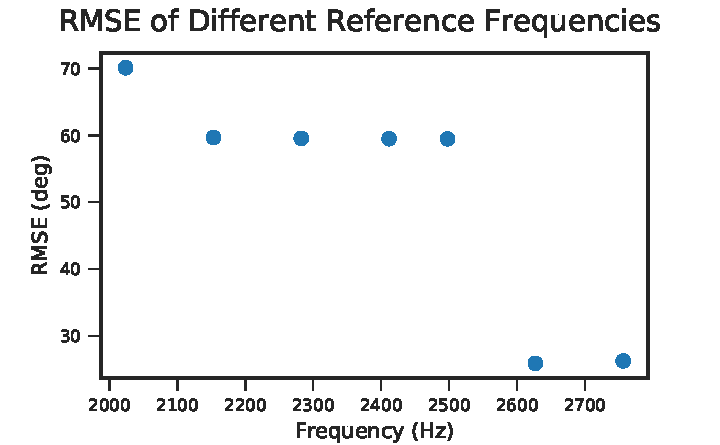
\includegraphics[]{figures/evaluation/phase_fc_rmse}
	\caption{Result of all measurements done with robot 26 to compare different
	fixed frequency values in whistle range.}
	\label{fig:04_diffFc}
\end{figure}
% -------------------------------------------------------------

On the basis of the results, the reference frequency was set to a minimum
of 2600\si{\hertz} for evaluation of the demonstration-dataset.
Hence, the reference frequency is 2627.1\si{\hertz} in the case of a \ac{FFT} length
of 256 samples.
Applying the phase difference method with this reference frequency, the final
direction estimate computed from the candidates listed in
\cref{tab:04_fixedFreqResult} is -29.6\si{\degree} which results in an error of
4.1\si{\degree}.
% -------------------------------------------------------------
\btline{ht}{1.2}
\btab{|c|c|c|c|c|}
\hline
Base Channel & Next Channel & Phase Difference & Candidate (-) & Candidate (+)\\
& & [\si{\deg}] & [\si{\deg}] & [\si{\deg}] \\
\hline
1 & 3 & -79.1 & -26.8 & 88.0\\
\hline
2 & 0 & 167.7 & -30.6 & -30.6\\
\hline
3 & 2 & 88.5 & -148.7 & -31.3\\
\hline
\etab
\et{Resulting candidates of phase difference method with fixed frequency
	2670.1Hz of example measurement from front right
	(-33.7\si{\degree})}{04_fixedFreqResult}
% -------------------------------------------------------------

\subsubsection*{Dynamic Reference Frequency Selection}

Another option is to have a nonspecific reference frequency that
is computed dynamically without a-priori knowledge.
As stated in the implementation chapter, frames are chosen where the frequencies
of the maximum amplitudes coincides for all channels.
For the running example discussed here, this corresponds to a frequency of 2756.25\si{\hertz}.

For comprehensibility, the determined frequency information visualized by
wave signals with the detected phases and amplitudes
in the lower subplot of \cref{fig:04_phaseSingle}.
In the upper plot of \cref{fig:04_phaseSingle} one sees the originally received microphone
data before applying a Hann window and transforming it into frequency domain by
\ac{FFT}. The resulting phases and amplitudes are listed in
\cref{tab:04_phaseSingle}.
% -------------------------------------------------------------
\begin{figure}[H]
	\centering
		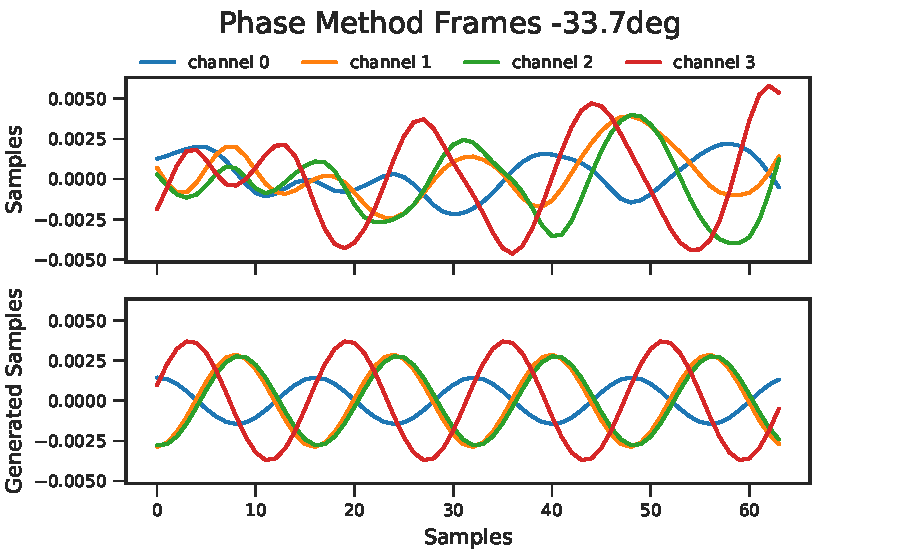
\includegraphics[]{figures/evaluation/phase_cos}
	\caption{Frames used for the direction detection by phase method.}
	\label{fig:04_phaseSingle}
\end{figure}
% -------------------------------------------------------------
\Cref{tab:03_maxFrequencies} pointed out that the most feasible frequency
of the rear channels 0 and 1 is not in whistle spectrum
due to the larger physical distance between the microphones.
Thus, the phase difference information is neglected because of the ambiguity of
the temporal sequence between the signals.
Following the procedure discussed in \cref{subsubsec:03_phase},
the resulting phase difference estimate
is -29.2\si{\degree} by combining the candidate direction -17.6\si{\degree},
-30.6\si{\degree} and -39.3\si{\degree} from channels 1, 2 and 3 according to
\cref{tab:04_phaseDiffSingle}.
% -------------------------------------------------------------
\btline{ht}{1.2}
\btab{|c|c|c|}
\hline
Channel & Phase [\si{\deg}] & Amplitude\\
\hline
0 & -1.55 & 0.00144\\
\hline
1 & -177.7 & 0.00287\\
\hline
2 & 173.4 & 0.00279\\
\hline
3 & -75.0 & 0.00372\\
\hline
\etab
\et{Phase and amplitude of frame signals with $f_c$ = 2756.25Hz}{04_phaseSingle}
% -------------------------------------------------------------
\btline{ht}{1.2}
\btab{|c|c|c|c|c|}
\hline
Base Channel & Next Channel & Phase Difference & Candidate (-) & Candidate (+)\\
& & [\si{\deg}] & [\si{\deg}] & [\si{\deg}] \\
\hline
1 & 3 & -102.7 & -17.6 & 78.8\\
\hline
2 & 0 & 173.4 & -30.6 & -30.6\\
\hline
3 & 2 & 113.1 & -140.7 & -39.3\\
\hline
\etab
\et{Phase differences and resulting direction candidates of demonstration-dataset
with dynamically determined reference frequency}
{04_phaseDiffSingle}
% -------------------------------------------------------------

\subsubsection*{Impact of Selected Frame}
\label{subsubsec:04_frameNumber}

Not only does the frequency play a major role for the phase method,
but also the samples chosen for analysis.
Again it is referred to the eleven measurements of the laboratory-dataset
recorded on the robot at the center point (no. 26).
To evaluate if and how the result changes over time, the selection window
is shifted by half the frame size from -5 shift steps to 20.
Recapitulating the implementation details for the static reference frequency case
in \cref{subsec:04_phaseSingle},
the first frame after the start index is chosen in which the whistle detection would
count a whistle signal.
This frame is represented by zero shift.

% [ 62.32629763  59.19634105  66.78950798  54.53898736  30.80692207
%   25.91537359  56.55427899  65.27548831  66.3898905   75.48670644
%   97.33965933  96.6373387  100.22012166 104.20160752  59.55737843
%   58.22148221  48.51237213  51.93254436  49.08273252  62.64453085
%   56.49506079  57.03430393  67.46509351  73.21671739  43.69704948]
In \cref{fig:04_phaseOverTime}, the resulting errors per shift
for all measurements are plotted, presenting the influence of the
selected frame around the signal start.
The reference frequency was set to 2627.1\si{\hertz} due to the
outcome that frequencies larger than 2600\si{\hertz} achieve best results.
The graph presents that frames nearest to the signal start reach best results
with an \ac{RMSE} of 25.9\si{\degree}.
These results show that the frame position has a significant influence on the prediction
accuracy of the direction detection.
Therefore, an accurate signal start detection is crucial for the preciseness of the \ac{SSL}
by phase difference.
% -------------------------------------------------------------
\begin{figure}[ht]
	\centering
		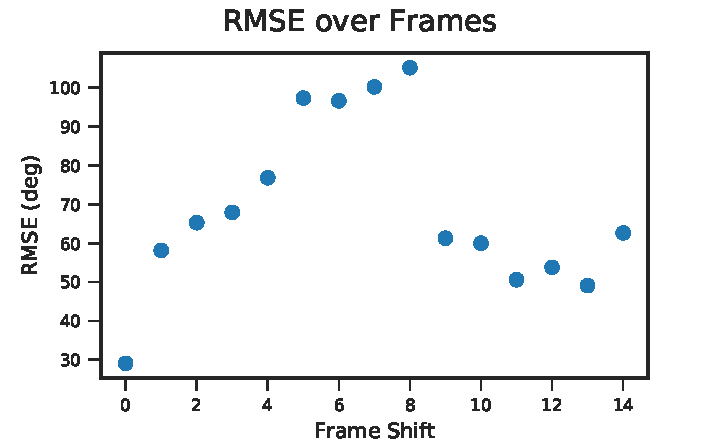
\includegraphics[]{figures/evaluation/phase_over_time}
	\caption{\ac{WSDE} result errors while shifting the frame over the
	samples of the laboratory-dataset on robot no 26.}
	\label{fig:04_phaseOverTime}
\end{figure}
% -------------------------------------------------------------

\subsubsection*{Phase Method Conclusion}
\label{subsubsec:04_phaseMethodConclusion}

Different options were investigated relating to the phase difference method
in the last subsections.
One finding is that reference frequency values should be chosen larger than
2.6\si{\kilo\hertz} for best results.
Another is that samples at the beginning of the signal are most suitable
for this method.
An advantage of the dynamically selected reference frequency is the reduction of
one parameter.
It requires more effort to implement and considering edge cases but
does not depend on the whistle detection.
Both approaches are valid for this work and result in a similar reference
frequency due to the limitations listed in \cref{subsubsec:03_phase}.

\subsection{\ac{TDOA} Method Comparison}
\label{subsec:04_singleRobotAngleError}

As the different \ac{TDOA} methods were discussed profoundly in the last
sections, all measurements of the laboratory-dataset are considered here
to make a generalized statement about the performance.
The \acp{WSDE} resulting from here are the inputs of the multi-agent
localization filter.
\Cref{fig:04_compareRmse} presents the \ac{RMSE} considering the
direction results of all five robots for each measurement in
\cref{subsec:04_labMeasurements}.
Additionally, the estimated standard deviation of each measurement
provides insight into the validity of the single robot results.
As one can see, the standard deviation of the relative angle of the \ac{GCC}
method is significantly smaller as compared to the phase method for most
measurements.
How this influences the reliability of the sound localization is
subject of discussion in \cref{sec:05_methodComparison}.
% -------------------------------------------------------------
\begin{figure}[h]
	\centering
		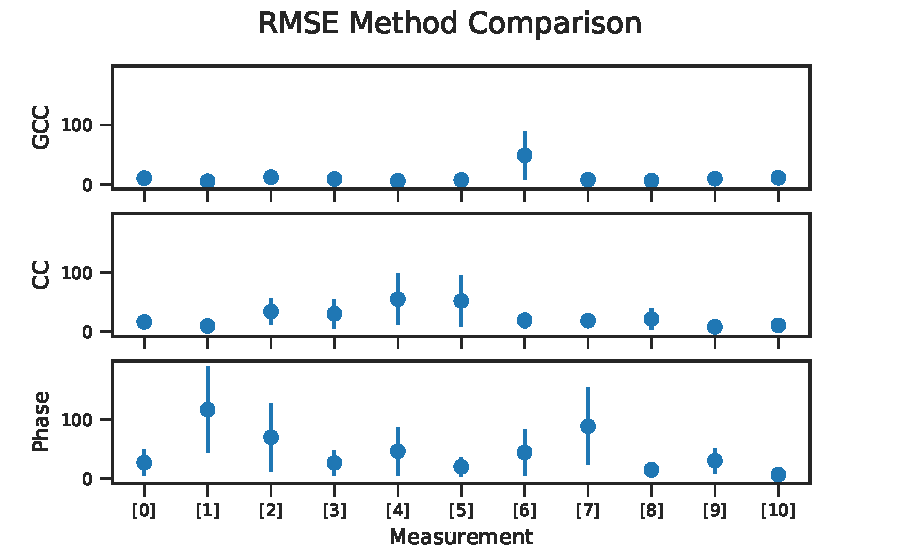
\includegraphics[]{figures/evaluation/compare_rmse}
	\caption{Angular RMSE and standard error of robot results per
	measurement of \cref{subsec:04_labMeasurements}.}
    \label{fig:04_compareRmse}
\end{figure}
% -------------------------------------------------------------

\subsection{Conclusion}
\label{subsec:04_tdoaConclusion}

The results in \Cref{subsec:04_singleRobotAngleError} show
that the \ac{GCC-PHAT} algorithm performs best according to the
laboratory-measurements.
Not only the errors are smallest, but also the low standard deviation
displays that the robots agree on the \ac{WSDE} and little outliers exist.
Also in regard to the multi-agent Bayesian updating filter, unified
results of the stand-alone robots are beneficial.
Another advantage of the \ac{GCC-PHAT} method is the presence of
a indication regarding the certainty of the measurement.
Interpreting the \ac{PSNR} as such, it can be used to detect outliers
or consider results with small \ac{PSNR} less.
\newpage
\section{Additional Information}
\label{sec:04_additionalInformation}
\todo[inline]{Not sure whether I mentioned earlier: "investigate" must be uesd carefully. You can say things like: "The performance of XYZ will be investigated." (but here I would also prefer "examined"). But you certainly can not say "XYZ will be investigated" because in this context "investigate" has more of a "legal" connotation.}

On top of the direction detection by \ac{TDOA}, additional information can be
extracted from the microphone data.
This information can be used to improve the single robot result or
to feed the team filter with beta\todo{beta or better? If beta: what does it mean?} information.
As \cref{sec:03_distance} has described, the distance of the sound source
can be estimated approximately for nearby signals that are aligned with
the x-axis of the robot's head.
Another intuitive approach is the inspection of the \ac{SNR} which
is expected to be higher for closer sound sources.
In addition, the \ac{PSNR} of the \ac{GCC} as defined in \cref{sec:03_snr} is examined.

\subsection{Distance Approximation}
\label{subsec:04_distance}

\Cref{sec:03_distance} presented the necessary conditions required to estimate the
distance of the sound source on a single robot.\todo{Please check whether this
sentence still states what you wanted to say. (Are you trying to say that under
certain conditions one can estimate the distance of the sound source from
a single robot? Or are you saying that certain conditions must hold for the
single robot to compute the distance from multiple robots (e.g. single robot
has to be able to resolve ambiguity of multiple candidates.))}
To examine the validity of these assumptions, measurements from the front and
back of the robot are collected and evaluated.
\Cref{tab:04_distance} lists the true distance as well as the distance estimate
for each measurement.
For both measurements with zero distance, the orientation of the whistle differed.
180\si{\degree} indicates that the whistle was turned in the opposite direction
of the robot.
In the other case (0\si{\degree}), the whistle was aligned with the robot.
The distance is represented in robot coordinates, so that positive distance
expresses that the source was placed in front of the robot and oriented towards it
and vise versa.
\todo[inline]{Maybe it would be good to use the same convention for all
measurements here. You could either annotate all measurements with an angle and
only positive distances or have a only a sign for all measurements (omit angle
for 0 as you can simply write +0 and -0) but have an explicit sign for all
measurements ( write +0.9 instead of 0.9)}
\todo[inline]{It might be more helpful to report errors here instead of the
estimates, but it's not a big problem if you leave it like this.}
\todo[inline]{I am guessing that for measurement 1 and 2 the true distance was
6 and 9 meters rather than 0.6 and 0.9 meters? Also, is there a reason why you
have more measurements from the back than from the front?}
% -------------------------------------------------------------
\btline{ht}{1.2}
\btab{|c|c|c|c|c|c|}
\hline
Nr. & True Distance [\si{\meter}] & GCC Result [\si{\meter}] & CC Result [\si{\meter}] & Phase Result [\si{\meter}]\\
\hline
1 & 0,9 & $\infty$  & $\infty$ & $\infty$ \\
\hline
2 & 0,6 & $\infty$ & $\infty$ & $\infty$ \\
\hline
3 & 0,3 & 0,35 & 0,25 &  0,13 \\
\hline
4 & 0,0 (180\si{\degree}) & -0,13 & -0,15 & -0,23 \\
\hline
5 & -0,0 (0\si{\degree}) & 0,22 & 0,21 & 0,02 \\
\hline
6 & -0,3 & -0,15 & -0,27 & -0,45 \\
\hline
7 & -0,6 & -0.34 & -0,50 & -0,62 \\
\hline
8 & -0,9 & -0.70 & -0,91 & -0,99 \\
\hline
9 & -1,2 & -1,00 & -1,28 & -1,71 \\
\hline
10 & -1,5 & -1,39 & -1,59 & -2,98 \\
\hline
11 & -1,8 & -1,72 & -2,07 & -3,33 \\
\hline
12 & -2,1 & -2,16 & $\infty$ & -3,02\\
\hline
13 & -2,4 & -2,31 & $\infty$ & $\infty$ \\
\hline
14 & -3,75 & -3,66 & -9,51 & -4,15 \\
\hline
15 & -6,4 & -7,35 & -7,27 & $\infty$  \\
\hline
16 & -9,8 & $\infty$ & $\infty$ & $\infty$ \\
\hline
\etab
\et{Result of front and rear distance for all methods.}{04_distance}
% -------------------------------------------------------------

As the results show, that in many cases the distance can be approximated with
adequate\todo{adequate rather means something like "hinreichend/ausreichend", maybe use "adequately
small error" oder "sufficiently small error"} error. One can see that the
\ac{GCC} results are erroneous for small
distances, but gives a correct approximation steadily.\todo{What do you mean by "steadily"?}
Compared to this, the \ac{CC} method performs better for small distances,
but fails completely for some measurements.
These failures of the \ac{CC} could be mostly attributed to cases where the
lateral delays exceeded the maximum lateral samples incorrectly.\todo{What do
you mean by "exceeded incorrectly", maybe drop "incorrectly"?}
The phase method provides most incorrect results.
Especially measurement 10 stands out by being double the real value.

\todo[inline]{Maybe you can show only the error statistics here and put the
real measurements in the appendix?}

For all measurements, the resulting direction angle of the sound source were
accurate.
\todo[inline]{For all measurements and all methods? Or does this statement only
hold for GCC? It seems like CC and Phase have some wrong predictions in 12 and
13}
Furthermore, the algorithm correctly detects sources that are out of
observable range.\todo{Is this the "observable range" or should this rather be
the "relevant range" (since these bounds seem to be imposed by SPL, not in
general)}

Unfortunately, for real cases one can not rely on the height parameter of the sound
source which varies from the referee's body height.
Having this as approximation only, the distance result should be handled
with care.

\subsection{SNR}
\label{subsec:04_snr}

Estimates of the uncertainty of a measurement can be utilized to inform the
Bayesian updating algorithm.
Depending on the uncertainty, the covariance matrix of the incoming result can
be adjusted so that predictions that are assumed to have higher error have
a smaller influence to the posterior estimate.
If a relation between received signal strength and distance to the source exists,
it would be a simple way to predict the sound source position roughly.
This can help for example, when team filter intersections are clustered so that
multiple location results exist.
% Thus, one intuitive hypothesis is assuming the existence of a relation between the
% received signal strength and distance to the source.

Taking the measurements of \cref{subsec:04_labMeasurements}, this hypothesis is
investigated by looking at the relation between distance and relative \ac{SNR}.
By reason of the whistle not blown equal for all measurements,
the \ac{SNR} is scaled by the overall mean of all robots' \acp{SNR} for one
measurement.
% $\text{Relative SNR} = \frac{SNR_{robot}}{Mean(SNR_{measurement})}$.
In \cref{fig:04_snrDistance} no straightforward
link between both values can be found unexpectedly.\todo{I would not write
"unexpectedly" here.}
\todo[inline]{Maybe report the correlation of these measurements. You can then
say, that SNR and Distance are only weakly correlated (small rho) which is
a bit more precise that using the "optisch gefuehlte Korrelation".}
% -------------------------------------------------------------
\begin{figure}[ht]
	\centering
	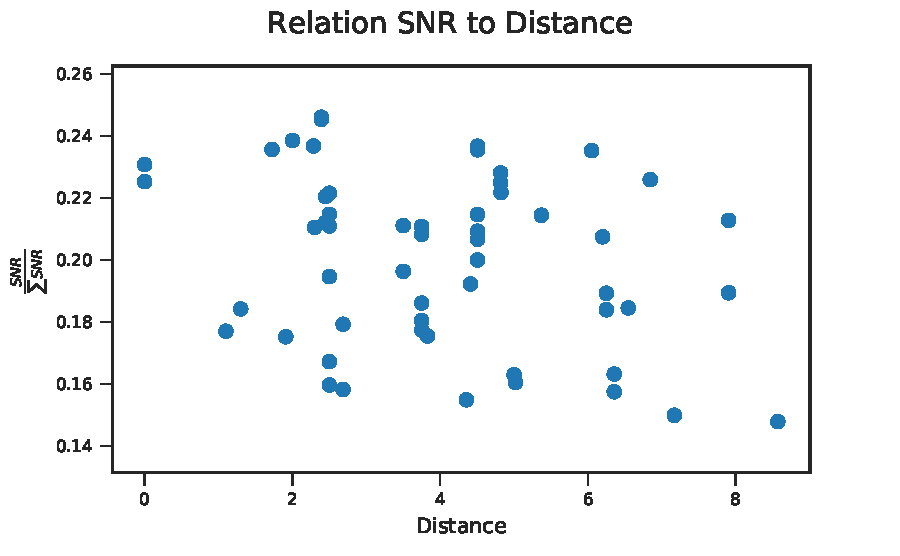
\includegraphics[]{figures/evaluation/snr_scatter}
	\caption{Visualization of relation between SNR and distance.}
	\label{fig:04_snrDistance}
\end{figure}
% -------------------------------------------------------------

Due to the result, further analysis on the \ac{SNR} values
on individual robots is done for evaluation of the microphones' validity.
\todo{How does this relate to your last sentence above? (I thought that the
conclusion was that things don't correlate?)}
For this purpose, a signal is played back digitally from fixed distance
and constant volume with different angles.
The main purpose of this measurement is to ensure that the individual channels
are not biased.\todo{Biased towards what?}
14 measurements of a 3\si{\kilo\hertz} sine signal
with are distance of 0.73\si{m} are done but no tendency is detectable.
Further evaluation is done by determining the channel with the maximum
\ac{SNR} of one measurement.
It is expected that the nearest channel to the sound source has maximum \ac{SNR}.
At 85,71\si{\percent} of the measurements this assertion could be
evidenced.\todo{How many measurements did you take?}
From this, it can be said that the general recordings of the microphones
are neither biased nor falsified.\todo{What do you men by falsified here?}
\todo[inline]{From the number of comments I put to this section I would
conclude that you could add a little bit more details on what the purpose of
this measurement was.}
\todo[inline]{IMHO a good practice is to report the number of experiments
and/or have the data in the appendix (if you still have the data). But having
it in the appendix is not super relevant. Don't waste time on it.}.

The same procedure is done with the real whistle recordings of the
measurement in \cref{subsec:04_labMeasurements}.
Using these measurements, only 54,55\si{\percent} of the maximum \acp{SNR}
match with the expected channels.
Consequentially, one must assume that the environmental circumstances
like multi-path propagation and reflection have large influence
on the signal data.
Thus, neither for a single robot direction result nor for the team filter
the \ac{SNR} can be utilized.

\subsection{PSNR}
\label{subsec:04_psnr}

As referred in \cref{sec:02_gcc}, the main characteristic of the \ac{GCC-PHAT}
algorithm is the emerging sharp peak.
In conclusion, one can assume that the lack of a sharp peak indicates
a less valid delay result of the \ac{GCC}.\todo{What is the reasoning behind
this conclusion? Maybe it is obvious to GCC familiar people but I fail to see
the causality.}
\todo[inline]{From this section introduction it is not clear what is happening in
this section. Maybe add a sentence on what is going to happen in 4.2.3 PSNR}

\subsubsection*{Informative Value}

This statement is examined by comparing the \ac{PSNR} value
to the error of the direction angle resulting from the \ac{GCC-PHAT} delay.
% Two cases of errors are taken into consideration.
In the following, the \ac{PSNR} is referred to as high if it exceeds 17,5
whereat the \ac{PSNR} value ranges from 10,1 to 28,8 for measurements in
\cref{subsec:04_labMeasurements}.

\todo[inline]{"Firstly" can not be used like this (it means "erstens" not
"zunaechst/zuerst"). Maybe grep through the document to make sure you don't use
it.}
First, for each channel pair the error between true direction and the most
suited direction candidate\todo{most suited according to which metric? The one
that is closest to the true direction or the one that has the "sharpest peak"?}
emerging from the \ac{GCC} delay.
The results are grouped into two classes based on the associated \ac{PSNR} value.
If the \ac{PSNR} of the \ac{GCC} is greater than the threshold of 17,5,
the \ac{RMSE} of its result is grouped to the errors with high \ac{PSNR}.
Elsewise, it pertains to the errors with low \ac{PSNR}.
This valuation is done with the measurements of \cref{subsec:04_labMeasurements}
and manually set start indices.
\todo[inline]{Maybe rather:"Out of a total number of X measurements,
Y correlations reported a PSNR below the threshold. The RMSE within this group
was 35.77\si{degree}".}
Having 76 correlations assessed with low \ac{PSNR}, the \ac{RMSE} of this group
is 35,77\si{\degree}.
Compared to this, the \ac{RMSE} of the remaining 144 measurements
is 15,86\si{\degree} only.
\todo[inline]{Always report what the RMSE belong to. E.g. here I can only
conclude from the unit that these are errors on the phase. But the context
sounds like they are errors on the PSNR.}

To see the impact on a complete robot result, the same is done
with the final angular errors of single robots results.
Here, the \ac{RMSE} of the lower \ac{PSNR} case results in 25,36\si{\degree}
whereat the error of the other case is 14,41\si{\degree}.
From this correlation between PSNR value and prediction accuracy one can
conclude that the PSNR is a useful indicator to inform about the validity of
direction estimates.\todo{Make sure that this sentence still says what you want it
to say.}

\subsubsection*{Frame Selection}

Another perspective is to include the PSNR information into the single
robot whistle direction estimation.
In \cref{fig:04_psnr2FrameShift}, the frame to investigate is
shifted before and after the signal start index.\todo{Signal start marked manually?}
Here, the same measurement as in \cref{sec:04_tdoaSingle} is used where
the robot was positioned at the center point
while the whistle is blown at -33,7\si{\degree} with 4,5\si{\meter}
distance.\todo{I would not cross-reference to another section here. Just
explain the experiment setup again as if it was a stand-alone experiment.
Jumping to other sections is annoying for the reader and it is not relevant to
know that you used the exact same data.}
The frame size of the \ac{GCC} is set to 256 samples and the shift
was set to a quarter of the frame size.
Samples of the rear left channel are plotted for better understanding
in the upper graph of \cref{fig:04_psnr2FrameShift}.\todo{Why "rear left" if
the signal comes from front right?}
The second graph shows the \ac{RMSE} of the robot direction result
over the frame shifts.
For the lower graph, the mean over the \acp{PSNR} of all channels
is presented.
As a general trend, it can be observed that the error of the predicted
direction is low for frame shifts with a high \ac{PSNR}. This again confirm the
hypothesis stated early in this section.
For shifts smaller than -2, the whistle signal does not intersect with the
evaluated frames. Therefore, the prediction error in this regime is high.
An important notice is that the \ac{PSNR} decays as the frame is shifted towards
later samples on the whistle signal. This indicates that the implemented
\ac{GCC-PHAT} method is not suitable for arbitrary subsamples of the signal.
% Without additional information about the rough direction,
% ambiguity exists due to periodicity of the signal.
% Due to the inconclusive result of the \ac{SNR} in \cref{subsec:04_snr}
% one decides not to take the signal magnitude as such information
% into account.
% Thus, the decisive role of the start of the signal is underlined again.
% -------------------------------------------------------------
\begin{figure}[ht]
	\centering
	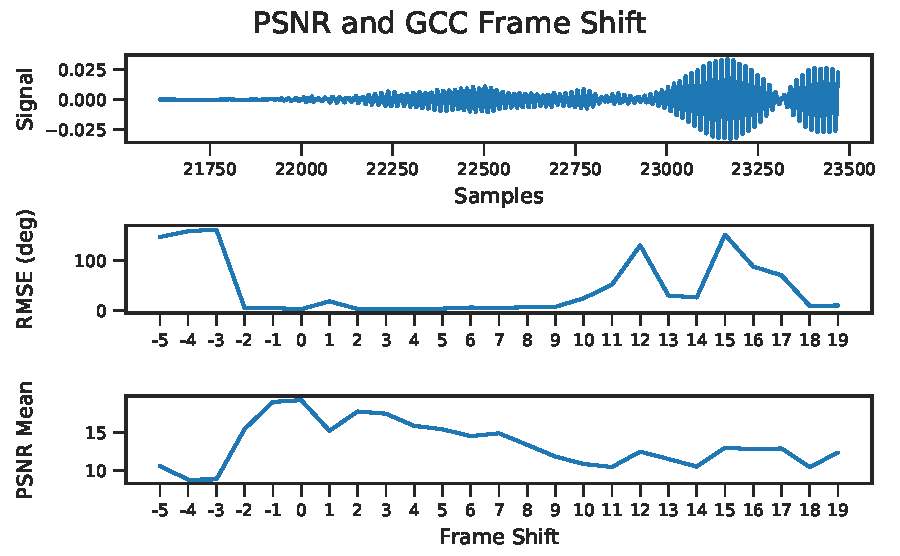
\includegraphics[]{figures/evaluation/gcc_frame_shift}
	\caption{
		Relation between \ac{PSNR}
		and selection of the frame in time. Signal data
		of the rear left channel is plotted in the upper window.
		In this measurement, the whistle is positioned at right front
		of the robot.
	}
	\label{fig:04_psnr2FrameShift}
\end{figure}
% -------------------------------------------------------------

\todo[inline]{Do you ever explicitly say how you end up using this information
in the team filter?}

\newpage
\todo[inline]{General, use pont instead of comma for numerical values}
\section{Team Evaluation}
\label{sec:04_teamEvaluation}

\todo[inline]{It took me a while to understand that you evaluate the team-performance
with all TDOA methods here. The introduction should point that out so that the reader
is not surprised. (see my comment on "why did you choose GCC)}

In the preceding sections of this chapter the performance of the three
\ac{TDOA} methods were evaluated with respect to the prediction accuracy on
individual robots.
The remaining part of this chapter focuses on the performance of the joint
whistle localization using measurements of multiple agents. \todo{Find
a consistent term to talk about "joint whistle localization"}
Input to the joint whistle localization are the direction estimates of each
robot in the team. Base on these results, the team whistle localization outputs
an absolute sound source position. To provide a decoupled result to the signal
start detection, the start indexes were set manually. \todo{for the entire chapter?}
\todo[inline]{(outdated, see comment at the beginning of this section) Which
TDOA method did you end up using here and why? Maybe there needs to be }

% It is looked at the result of one exemplary measurement where the behavior
% of the team filter is of prime importance.


\subsection{GCC Method}
\label{04_teamGcc}

To determine an overall result, each robot computes a direction prediction from
the locally recorded signal using the \ac{GCC-PHAT} method standing
alone.\todo{I feel like the conclusion of "what is the best TDOA method" needs
to be before this section. Otherwise it is not clear why you use GCC-PHAT here}
These local direction estimates of individual robots are fed to the team
decision filter as specified in \cref{sec:03_teamDecision} which estimates the
global sound source position by combining all measurements through Bayesian
updates.

For further clarification, measurement 1 of \cref{subsec:04_labMeasurements} is
presented in greater detail as an example.
\Cref{fig:04_gccResult} illustrates the result of the relative direction
estimates $\gamma$ of the individual robots listed in \cref{tab:04_gccResult}
for this example.\todo{Maybe gamma should have a lower index}
For \cref{fig:04_setup,fig:04_gccResult}, robot positions are marked by yellow dots
where a short yellow line indicates each robot's orientation.
The arrows in \cref{fig:04_gccResult} represent the local direction estimates
$\gamma$ as predicted by each robot. Finally, the true position of the sound
source is marked with a red star while the joint position estimate over all
robots is visualized by a cross.
% -------------------------------------------------------------
\btline{ht}{1.2}
\btab{|c|c|c|c|}
\hline
NAO & $\gamma$ [\si{\deg}] & Abs. Error [\si{\deg}] & Mean PSNR \\
\hline
21 & -26.22 & 3.71 & 18.3\\
\hline
24 & -133.77 & 9.32 & 16.8\\
\hline
26 & -30.19 & 3.50 & 19.6\\
\hline
27 & -75.26 & 1.71 & 17.4\\
\hline
28 & -15.90 & 2.53 & 15.1\\
\hline
\etab
\et{Resulting direction estimates of the individual robots with \ac{GCC-PHAT}
method for a whistle sound signal in the right front corner of the playing
field}{04_gccResult} \todo[inline]{Does Abs Error refer to the true error or
the estimated error (e.g. uncertainty).}
% -------------------------------------------------------------
\begin{figure}[ht]
	\centering
		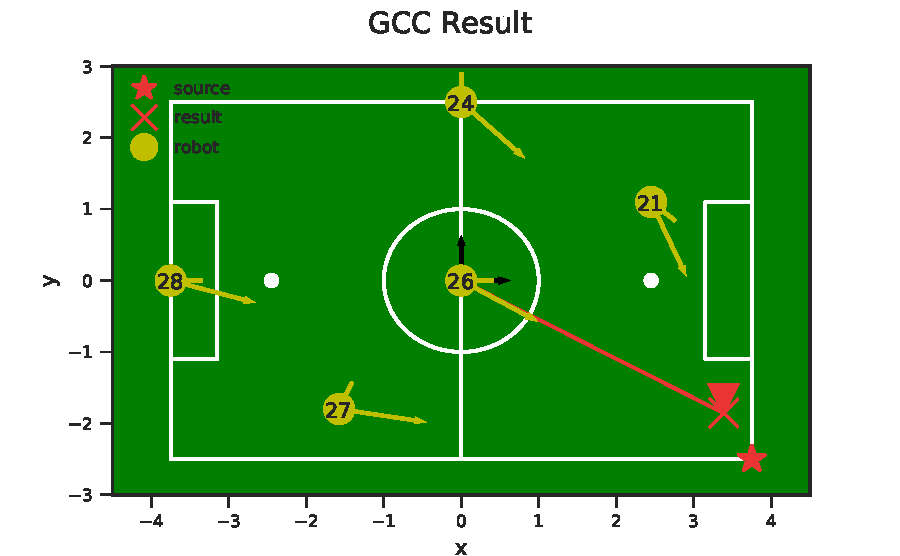
\includegraphics[]{figures/evaluation/gcc_team}
	\caption{Team whistle localization result with \ac{GCC-PHAT}
	method.}
    \label{fig:04_gccResult}
\end{figure}
% -------------------------------------------------------------

The final result and its corresponding errors are listed in
\cref{tab:04_gccTeamResult}. With an absolute distance error of less than
1\si{\meter} and small angular error, the source localization works
sufficiently for this case of application.
% -------------------------------------------------------------
\btline{ht}{1.2}
\btab{|c|c|c|}
\hline
 & Result & Error\\
\hline
Position x [\si{\meter}] & 3.38 & -0.37\\
\hline
Position y [\si{\meter}] & -1.85 & 0.65\\
\hline
Angle & 33.18\si{\degree} & 1.57\si{\degree}\\
\hline
Distance [\si{\meter}] & 3.85 & 0.74 \\
\hline
\etab
\et{Whistle localization result of measurement 1 with \ac{GCC-PHAT} method}{04_gccTeamResult}
% -------------------------------------------------------------

\Cref{tab:04_gccTeamResult} shows the distance and angle errors
for all measurements in \cref{subsec:04_labMeasurements}.
The \ac{RMSE} in distance being 0.87\si{\meter} and angular \ac{RMSE}
being 5.07\si{\degree} one can say that the \ac{GCC-PHAT} algorithm
works well for whistle sound source localization.
% -------------------------------------------------------------
\btline{ht}{1.2}
\btab{|c|c|c|c|c|}
\hline
Measurement & Error x [\si{\meter}] & Error y [\si{\meter}] & Abs. Distance Error [\si{\meter}] & Angle Error\\
\hline
0 & 1.31 & 1.06 & 1.68 & 1.45\si{\degree}\\
\hline
1 & 0.13 & 0.06 & 0.15 & 1.57\si{\degree}\\
\hline
2 & 0.59 & 0.43 & 0.73 & 0.42\si{\degree}\\
\hline
3 & 0.54 & 0.47 & 0.72 & 9.09\si{\degree}\\
\hline
4 & 0.27 & 0.0 & 0.27 & 0.01\si{\degree}\\
\hline
5 & 0.15 & 0.14 & 0.21 & 3.18\si{\degree}\\
\hline
6 & 0.41 & -0.02 & 0.41 & 2.67\si{\degree}\\
\hline
7 & 0.39 & 0.02 & 0.39 & 8.98\si{\degree}\\
\hline
8 & 1.84 & -0.01 & 1.84 & 0.14\si{\degree}\\
\hline
9 & 0.58 & 0.52 & 0.78 & 9.89\si{\degree}\\
\hline
10 & 0.03 & -0.0 & 0.03 & 0.0\si{\degree}\\
\hline
\etab
\et{Whistle localization results for all measurements in \cref{subsec:04_labMeasurements} with
\ac{GCC-PHAT} method}{04_gccTeamResult}
% -------------------------------------------------------------
% - intersections
% - updates
% - covariance
% - PSNR

% -------------------------------------------------------------
\subsection{CC Method}
\label{04_teamCc}

The \ac{CC} method is evaluated on the same data as in
\cref{subsec:04_labMeasurements}.\todo{You should probably just say this once
in the beginning (e.g. all evaluations use the same dataset).}
The results for the predictions of this method are reported in
\cref{tab:04_ccTeamResult}. Over all measurements, the \ac{CC} predictor has
a \ac{RMSE} of 1.45\si{\meter} in distance and 10.67\si{\degree} angular. The
results show that the standard \ac{CC} performs worse as compared to the
\ac{GCC-PHAT} method. Indeed, the statements in \cref{sec:02_cc} prove to be
true.

% -------------------------------------------------------------
\btline{ht}{1.2}
\btab{|c|c|c|c|c|}
\hline
Measurement & Error x [\si{\meter}] & Error y [\si{\meter}] & Abs. Distance Error [\si{\meter}] & Angle Error\\
\hline
0 & 0.6 & 1.39 & 1.51 & 8.15\si{\degree}\\
\hline
1 & -0.49 & 1.2 & 1.3 & 11.97\si{\degree}\\
\hline
2 & 2.32 & 2.11 & 3.13 & 18.28\si{\degree}\\
\hline
3 & 1.07 & -0.96 & 1.44 & 3.71\si{\degree}\\
\hline
4 & 1.95 & -0.09 & 1.95 & 10.44\si{\degree}\\
\hline
5 & 0.07 & 0.01 & 0.07 & 0.32\si{\degree}\\
\hline
6 & 0.4 & -0.01 & 0.4 & 1.91\si{\degree}\\
\hline
7 & 1.06 & -0.0 & 1.06 & 22.99\si{\degree}\\
\hline
8 & 1.24 & -0.06 & 1.24 & 0.77\si{\degree}\\
\hline
9 & -0.04 & 0.78 & 0.78 & 7.22\si{\degree}\\
\hline
10 & 0.03 & -0.0 & 0.03 & 0.0\si{\degree}\\
\hline
\etab
\et{Whistle localization results for all measurements in \cref{subsec:04_labMeasurements} with
\ac{CC} method}{04_ccTeamResult}

Further information about the source of the error can be obtained
by looking at the single robot results of each measurement.
Since the team filter is updated computing the intersections of the
individual robot's direction estimates, the accuracy of the absolute position
depends on the number of arising intersections.\todo[inline]{It is not immediately
clear whether "more intersections" is better or worse.}
This will be discussed in \cref{subsec:04_singleRobotAngleError}.
% -------------------------------------------------------------
\subsection{Phase Method}
\label{04_teamPhase}

Finally, the performance  of the phase method is evaluated. For this
experiment, the minimal frequency value parameter is set to
2700\si{\hertz}.\todo{Is this even relevant? It seems like it does not add
information, unless you justify why this is a good choice of parameters. I would
drop it.}
The results of phase method for this experiment are shown in
\cref{tab:04_phaseTeamResult}.
The \ac{RMSE} of the position estimate is close to the prediction accuracy of
the \ac{CC} method with 1.33\si{\meter}.
The \ac{RMSE} of global direction estimate of 74.8\si{\degree}
shows a significantly worse performance than the other two methods.
However, it must be noted that these angular error mainly arise from
measurements 6 and 10. Both measurements are taken at the center point of the
field. Since the absolute position is in an acceptable error range, these
angular results will be treated as outliers for the error calculation. Thus,
the angular \ac{RMSE} of the phase method without measurements 6 and 10 is
11.69\si{\degree}.\todo{Does it even make sense to report the angular error for
the team estimate? This has weirdly non-linear as the error statistics
essentially have a singularity at 0. It does not even seem to be well defined
what should be the "true orientation" if the whistle is blown at 6 or 10. Any
direction would be correct for this case.}

% -------------------------------------------------------------
\btline{ht}{1.2}
\btab{|c|c|c|c|c|}
\hline
Measurement & Error x [\si{\meter}] & Error y [\si{\meter}] & Abs. Distance Error [\si{\meter}] & Angle Error\\
\hline
0 & -1.07 & -0.98 & 1.45 & 4.13\si{\degree}\\
\hline
1 & 0.21 & 0.27 & 0.34 & 4.27\si{\degree}\\
\hline
2 & 0.22 & 1.39 & 1.41 & 16.25\si{\degree}\\
\hline
3 & 1.26 & -0.02 & 1.26 & 11.19\si{\degree}\\
\hline
4 & 0.16 & -0.04 & 0.17 & 0.99\si{\degree}\\
\hline
5 & -0.42 & 0.19 & 0.47 & 5.46\si{\degree}\\
\hline
6 & -0.32 & 0.08 & 0.33 & 166.25\si{\degree}\\
\hline
7 & -0.28 & 1.76 & 1.78 & 20.82\si{\degree}\\
\hline
8 & 2.37 & 0.27 & 2.39 & 4.23\si{\degree}\\
\hline
9 & 2.04 & 0.29 & 2.06 & 24.89\si{\degree}\\
\hline
10 & -0.32 & 0.0 & 0.32 & 180.0\si{\degree}\\
\hline
\etab
\et{Whistle localization results for all measurements in \cref{subsec:04_labMeasurements} with
phase method}{04_phaseTeamResult}

% Another point to take into account is the number of intersections
% yielded in the team filter from the direction rays.
% Compared to 
% more robots that fail -> less intersections
% show number of intersections for each file compared to method
% The rest of algorithm as presented in 03 phase

\section{Signal Start Detection}
\label{sec:04_signalStartDetection}

\todo[inline]{This section seems a bit misplaced. I feel like "Team Evaluation"
should be the last evaluation section. Is there a reason why you can't put this
before that?}

In previous chapters, the importance of the signal start was emphasized.
% Due to the fact that the direction detection methods is
% executed on smaller frames than the actual whistle detection.
% To demonstrate this for the phase method, the frame to examine is
% shifted with time \cref{subsec:04_frameNumber}.
Especially the result in \cref{subsec:03_phase} has shown that in fact, the
accuracy of the direction predictor decreases when evaluated on later samples
of the whistle signal.\todo{Maybe interpret this somewhere: give a reason
why shit makes sense (e.g. maybe because more reflections of the signal will
have reached the microphone)}
Also according to the outcome of \cref{subsec:04_psnr}, the \ac{GCC}
method performs best with frames near to the signal start. \todo[inline]{Get
rid of some cross-references and/or write more about what happened in these
chapters. (I don't remember what happened in 3.4 and 4.2.3 and jumping back and
forth is annoying.)}

% There are some reasons why other methods were tested to find the signal start.
In order to find a good solution for a highly reliable, accurate but
computationally tractable start detection, different approaches were
tested profoundly.
For high temporal\todo{I added "temporal" here because otherwise it seems unintuitive
that a less samples is better (because at the same time it might be harder to
predict from fewer samples as there is less information in the frame)} accuracy
either the number of samples in a frame have to be small\todo{Maybe rather say
that the frame as to be small? A low number of samples in a frame could also be
achieved by a smaller sampling rate, which would not help.} or the window must
be shifted with small steps which both implicit a large number of evaluations.
The existing whistle detection algorithm of the HULKs presented in
\cref{subsec:03_whistleDetection} is computationally intensive and has a low
accuracy for small frames\todo{Is "frames" actually the correct term (in
general)? Shouldn't it be "window"? I don't know what people use in signal
processing literature} as shown in \label{subsec:04_whistleDetection}.
Therefore, the goal is to identify a\todo{"looked" doesn't work this way. You are using this
quite a lot. Maybe grep the document for it and replace it.} simple algorithm for
the signal start detection. Ideally, this algorithm should be adaptable to
signals other than the whistle sounds.\todo{I would add a reference to the section
where you presented these algorithms. (this is only the evaluation, right?)}

Hereinafter, the performance of each method methods is evaluated by
analyzing the error between algorithmically determined start index
and manually labelled start index.
As a benchmark, the prediction accuracy is evaluated on 11 measurements on all
robots\todo{how many robots?} \todo{this sentence is missing some
words}\cref{subsec:04_labMeasurements}.
By the frame size of the \ac{FFT} being set to 256 samples for the
correlation methods, a start index error of at most 256 samples is
desired.
Therefore, a start index detection result is regarded as failure for errors
larger than 256 for the following sections.
Two metrics are specified to express the degree of failure.
The former counts the number of large errors for each channel.
In this case, 220 sample data for 11 measurements on five robots with
four channels each exist.\todo{I don't understand this sentence.}
The second metric reports the number of measurements for which any of the
channels failed. For this case, 55 measurements are given.\todo{Again, what is
this sentence saying? I thought we had 11 measurements? Or is it 11
measurements * 5 robots? Maybe simply write 55 in the first place (rather than
11)}.
% -----------------------------------------------------------------------------------------------------

\subsection{Whistle Detection}
\label{subsec:04_whistleDetection}

\todo[inline]{It is not immediately clear that with "whistle detection" you refer
to the "whistle detection of the HULKs", e.g. your "baseline"}
First, the accuracy of the whistle detection in regard of the start index
is evaluated.
Here, the start index is defined as the first index where the whistle detection
found a whistle.
With a frame size of 1024, the whistle detection algorithm fails in every of the
55 measurements with at least one channel if only an error of at most 256 samples
is permitted.
However, every error is in the range of 1024 samples which proves that the
approximate start of the whistle sound is detected correctly.
With a smaller frame size of 256, the temporal accuracy is improved but
introduces false positive detections.\todo{do you have numerical results here?}
With the results, one can say that the whistle detection is not sufficient
for the start detection or is at least not reliable as stand-alone solution.
Furthermore, this approach is limited to sounds in fixed and known frequency range.
%  failure rate of
% 9\si{\percent} in regard to every channel.
% In this work microphone data were saved as soon as the whistle detection module
% found a whistle sound in the audio samples.
% Due to this implementation, the algorithm does never fail to detect the whistle
% Standing alone, the error is always in the range of \si{\pm1024} samples due to the
% set frame size of 1024 samples.
% With a smaller frame size of 256, the accuracy gets better with an error of
% 9\si{\percent} in regard to the 220 sample data but has an error rate of
% 25,5\si{\percent} for the measurements.

% looking at the next 300
% values and with a step size of 50 the result is 15\si{\percent} and 36\si{\percent}
% and with step size 1, it is 13\si{\percent} and 33\si{\percent}.
% This is computationally very costly and the reward is small.

\subsection{ZCR}
\label{subsec:04_zcr}

For the evaluation of the \ac{ZCR},
the frame size is set to 256 samples and number of noise and signal frames
are set to 10 frames.
In 7\si{\percent} of the 220 channel sample data\todo{"sample data" sounds like
it is not a term. Maybe only "samples"?}, the method fails with a significant
error larger than 256 samples.\todo{I don't thing you have to repeat the 256
sample criterion every time. You defined what is considered a failure earlier.
Just say "failed".} In most cases, the method provides accurate results with
small error. Taking all measurements of robot 26 as example, the \ac{RMSE}
amounts 54.23 samples.\todo{Again, where is the data for this? Tables, figures?}

However, there are cases where the algorithm fails. Looking at those cases it
could be identified that the errors occur often due to incorrect assumptions
that the signal is present at the end of the buffered samples.
Some measurements prove that this is not always the case as shown in
\cref{fig:04_zcrFail}.
Here, the data of the front right channel of robot 21 with the whistle source
at position 5 in \cref{subsec:04_labMeasurements}
illustrates how the signal ended around 35000 samples already. \todo{Neither
the robot number, nor the position or the channel are relevant here I think.}
If the start index is determined at the point where the \ac{ZCR}
falls below the threshold searching backwards as stated in \cref{sec:02_signalStartDetection},
the detection fails.

In most cases, only one out of four channels produces a erroneous
result.\todo{Why? Doesn't the signal end early on all channels?}
Because the final start index on one robot is set equal for all channel,
the failure can be compensated with a simple voting procedure.
% -------------------------------------------------------------
\begin{figure}[ht]
	\centering
	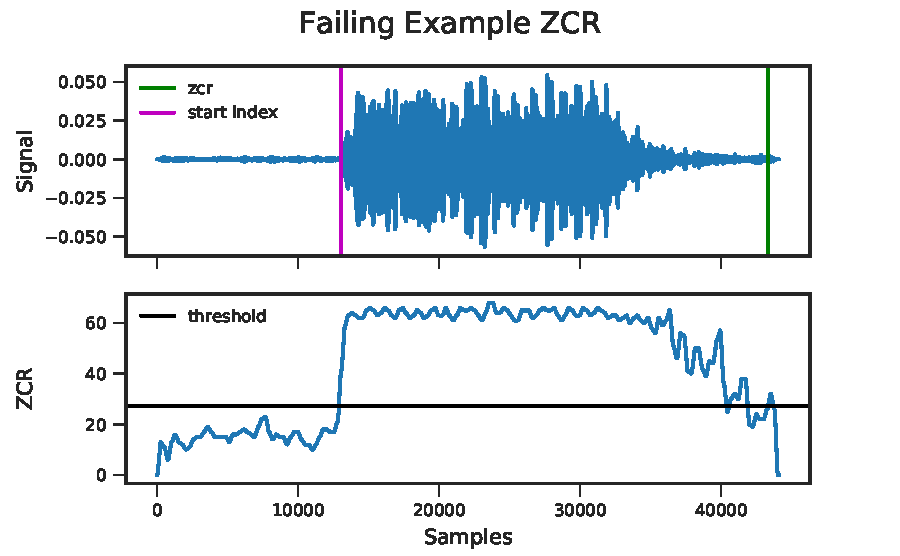
\includegraphics[]{figures/evaluation/zcr_fail}
	\caption{Channel 3 data from measurement 5 of \cref{subsec:04_labMeasurements}
		for robot number 21. A failing example for the start detection by \ac{ZCR}
		is shown.}
	\label{fig:04_zcrFail}
\end{figure}
% -------------------------------------------------------------
If the start index is determined at the point where the \ac{ZCR}
falls below the threshold searching backwards as stated in \cref{sec:02_signalStartDetection},
the detection fails.

In most cases, only one channel of four output a erroneous result.
Because the final start index on one robot is set equal for all channel,
the failure can be compensated with a smart voting procedure.

Another option exists by changing the process of finding the
threshold excess onwards.\todo{I don't understand what this is saying.}
In this case, the threshold is scaled with a factor of 1.25.
Results by this were poorer than the initially implemented manner
with a failure rate of 15\si{\percent}.\todo{Did you ever report the previous failure rate?}
By adding the constraint that multiple samples must exceed the
threshold successively, result can be slightly improved for the cost of higher
computational effort.

It should be noted that the poor performance of the \ac{ZCR} method with signal that
was cleaned with spectral subtraction previously. This surprising outcome is
convenient for the overall task, because the start index result can be embed
into the spectral subtraction, providing information for separating the noise
and signal part.\todo{I don't get what this paragraph is saying?}

\subsection{Entropy}
\label{subsec:04_entropy}

As discussed in \cref{subsec:02_Entropy} the entropy quantifies the amount
of chaos in a signal frame.\todo{Is this correct? Chaos is deterministic and not
the same as randomness}
Especially for signals to localize with unknown characteristics,
this method can be useful because no a-priori knowledge is needed.\todo{You should
probably say that the only prior knowledge must be, that the signal to detect
has lower entropy than the background noise.}
For all measurements this method yielded poorer results than the \ac{ZCR} method
with a failure rate of around 20\si{\percent}.
Best results are achieved with a frame size of 512 samples and a step size of 800
samples.
% \change[]{Explain what steps are? Maybe in implementation?}
However, for records with fading whistle the entropy method
generates more reliable results than the \ac{ZCR} method.\todo{What do you mean
by "fading whiste"? Whistles that don't have a distinct/abrupt start?}
Taking the same measurement as an example for which failure of the \ac{ZCR} method
was discussed earlier, \cref{fig:04_entropyGood} shows how the algorithm
detects the signal start correctly even though the whistle sound ended at
around 35000 samples. In this measurement, the start index errors of all four
channels were smaller than 40 samples.
% -------------------------------------------------------------
\begin{figure}[ht]
	\centering
	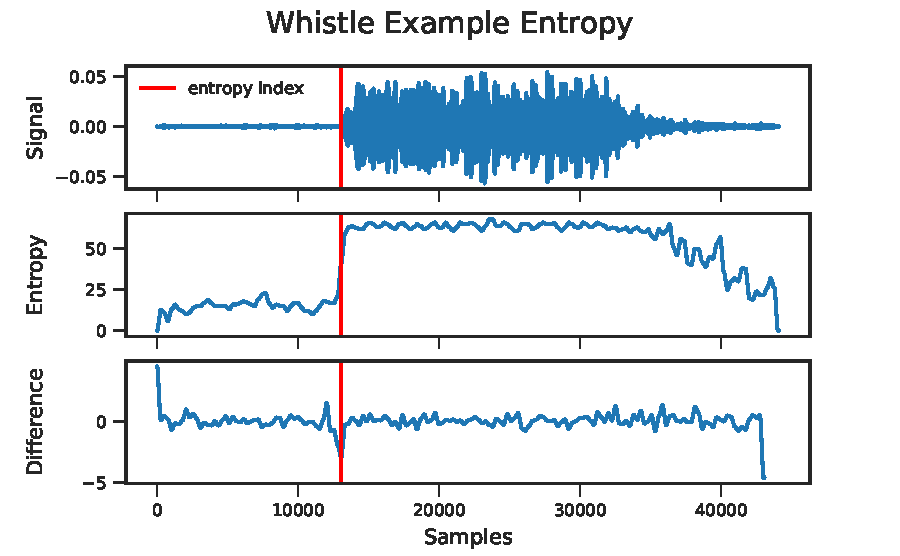
\includegraphics[]{figures/evaluation/entropy_good}
	\caption{Exemplary result of start index detection by entropy where
			the \ac{ZCR} method failed due to fading whistle
			at the data.}
	\label{fig:04_entropyGood}
\end{figure}
% -------------------------------------------------------------

% But as the entropy should be larger for noisy environment
% performance in other surrounding of measurement at \ac{RoboCup} is looked at.
% Entropy would be best for undefined signal -> distinguish between
% signal and noise without information


\todo[inline]{General, use pont instead of comma for numerical values}